\section{Optical Character Recognition}

\begin{frame}{Bearbeitungsschritte}
    \begin{columns}
        \begin{column}{0.6\textwidth}
            \begin{enumerate}
                \item {\small Vergr\"osserung und Graustufen}
                \item {\small Blurring (Bildgl\"attung)}
                \item[-] {\scriptsize Gaußsche Unsch\"arfe und Median Unsch\"arfe}
                \item {\small Thresholding (Schwellenwertverfahren)}

                \item[-] {\scriptsize Otsu: w\"ahlt automatisch einen geeigneten Schwellenwert aus}
                \item[-] {\scriptsize Einfaches Verfahren mit Schwellenwerten $\{60,80,100,120\}$}
                \item[-] {\scriptsize Binary-Inv.: Die Werte derart getauscht, dass schwarz zu weiß wird und umgekehrt $\rightarrow$ führt zur besseren Erkennung von Konturen}

                \item {\small Dilation (Morphologische Transformation)}
            \end{enumerate}
        \end{column}
        \begin{column}{0.40\textwidth}
            \begin{center}
                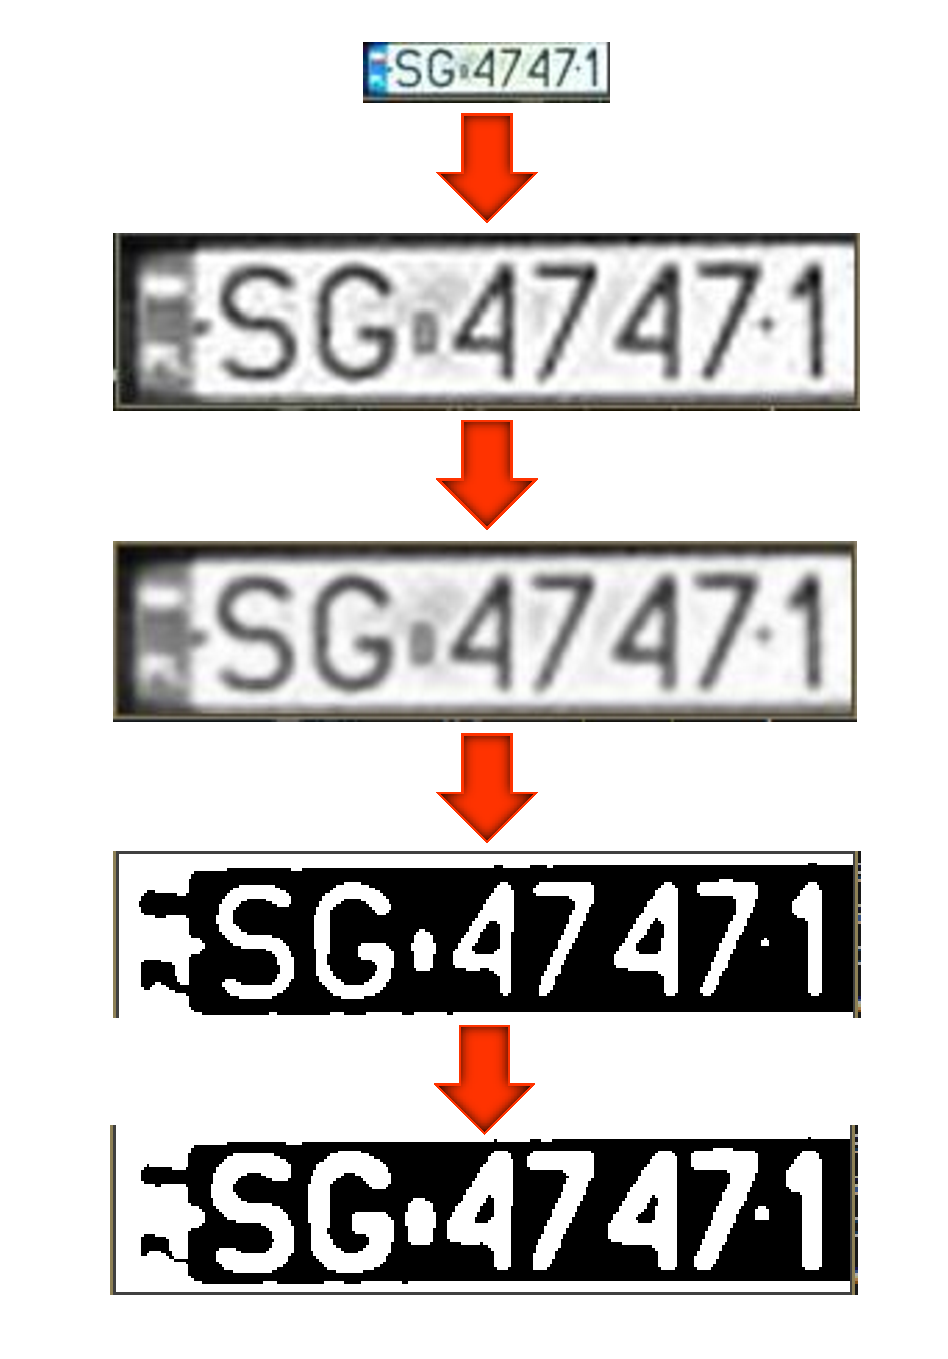
\includegraphics[width=\textwidth]{img/preprocessing}
            \end{center}
        \end{column}
    \end{columns}
\end{frame}

\begin{frame}{Aussortierung der Konturen}
    \begin{itemize}
        \item {\textit{\scriptsize Genutzt werden die Werte x, y, w, h (Werte der Kontur) sowie width und height (Breite und Höhe des Bildes)}}
        \item {\scriptsize Es werden nur Konturen berücksichtigt, die folgende Bedingungen erf\"ullen:}
    \end{itemize}
    \begin{align*}
        \frac{height}{h} > 3
        \hspace{1cm}
        \frac{h}{w} < 1.2
        \hspace{1cm}
        \frac{width}{w} > 50
    \end{align*}
    \begin{center}
        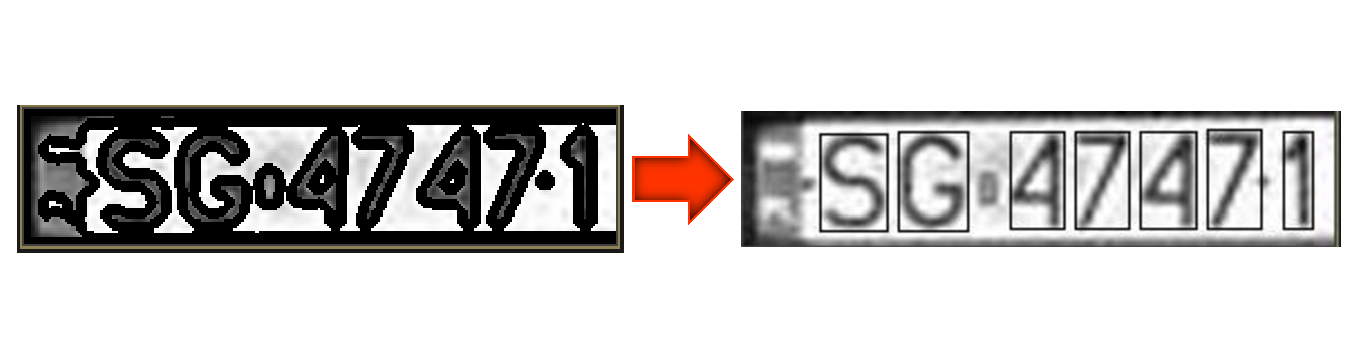
\includegraphics[width=\textwidth]{img/contours}
    \end{center}
\end{frame}

\begin{frame}{Character auslesen}

    {\footnotesize Einstellungen für das Auslesen mit Tesseract 5:}
    \begin{itemize}
        \item {\scriptsize Jeder Character wird einzeln ausgelesen \rightarrow  \, Page Segmentation Mode (\texttt{--psm10})}
        \item {\scriptsize Engine Mode \texttt{--oem3}}
        \item {\scriptsize Zeichen-Whitelist (Großbuchstaben + Zahlen 0-9)}
        \item {\scriptsize Außerdem: Bild darf nicht zu nahe am Character ausgeschnitten werden}

              \begin{center}
                  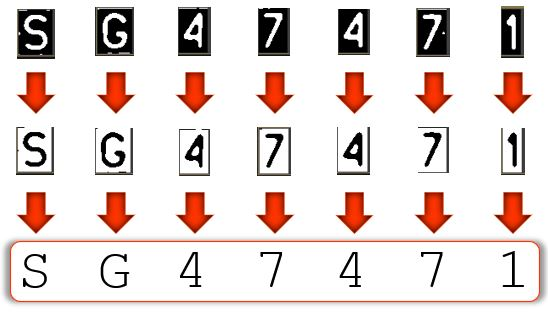
\includegraphics[width=0.75\textwidth]{img/char_preprocessing.jpg}
              \end{center}

    \end{itemize}
\end{frame}


\begin{frame}{Boundingboxes verschieben}
    Falls keine Character in der gefundenen Bounding-Box erkannt werden, verschiebe die Bounding-Box anhand unterschiedlicher Methoden: {\textit{hoch, runter, rechts, links, oben-rechts, unten-rechts, unten-links, oben-links}}
    \begin{center}
        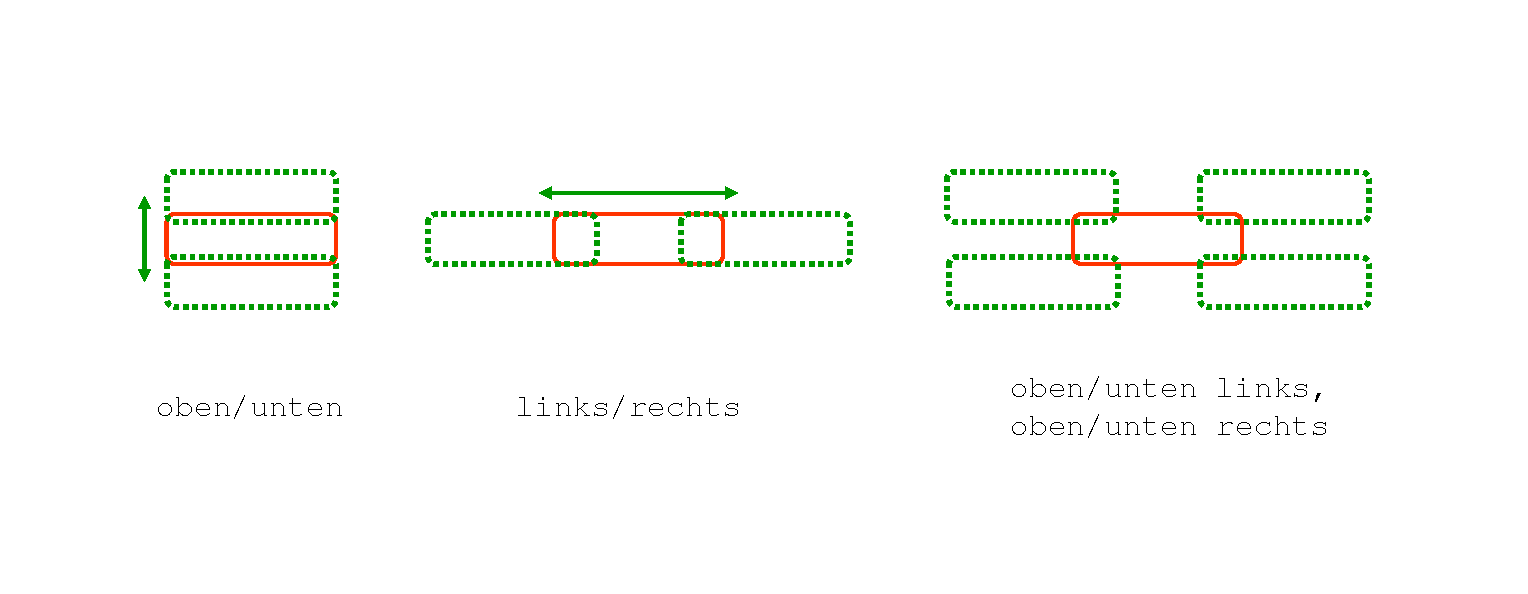
\includegraphics[width=\textwidth]{img/bbox_shift}
    \end{center}
\end{frame}

\begin{frame}{Levenshtein-Distanz}
    \begin{table}[H]
        \centering
        \caption{Levenshtein-Distanz}
        \begin{tabular}{ccc}
            ohne Verschiebung & mit Verschiebung & mit Verschiebung           \\
                              &                  & \& Thresholding-Variierung \\
            4.05              & 3.55             & 3.2
        \end{tabular}
    \end{table}
\end{frame}

